

\section{Mean power (Have to use a better title than this)}

Mass ratio ($m^*$) and damping ratio($\zeta$) was treated as two different variables in the presentation of data. Fig.  \ref{fig:power_barrero_style_zeta_165} and \ref{fig:power_barrero_style_mstar_165} shows the mean power against $U^*$ at different $\zeta$ and  $m^*$. The data in Fig \ref{fig:power_barrero_style_zeta_165} seems to agree qualitatively with \cite{Barrero-Gil2010a} where the peak power was shifting when the damping ratio increased. An interesting observation is that the peak power remains to be constant regardless of the damping ratio where \cite{Barrero-Gil2010a} also observed and concluded that the maximum efficiency attainable does not depend the $m^*\zeta$ parameter. A similar observation was made when $m^*$ was increased (Fig.\ref{fig:power_barrero_style_mstar_165}). However, the peak power at $m^*=20$ was lesser than the other mass ratios ($m^*=30,40,60$) which produced the same peak mean power. This may be due to the effect of shedding. \cite{Joly2012}  an influence of vortex shedding on galloping amplitude at low mass ratios. The data obtained using \cite{Parkinson1964} $C_y$ curve shows a similar pattern (Fig.\ref{fig:power_barrero_style_zeta_Park}) where a common maximum power could be observed. Hysteresis could be observed in the power curves.
The mean power data at different damping ratios could be collapsed by changing the independent variable form $U^*$ to the $\text{damping factor}= \frac{4\pi\zeta m^*}{U^*}$ Fig.\ref{fig:mean_power_collapsed_c_with_FSI}. This phenomenon could also be observed when the mean power data at different mass ratios plotted in the earlier mentioned independent variable.


An explanation for this could be provided using an energy point of view. The power generally could be expressed as the product of force and velocity. Therefore  the product of the  force exerted by $C_y$ and the velocity of the body $\dot{y}$, could be expressed as the power transfer from fluid to body (disregarding minor losses). On the other hand by using the term $(c\dot{y})\dot{y}$  the dissipated power due to mechanical damping of the system could be obtained.

As an example time histories of both dissipated power and the transferred power are presented in 3 different reduced velocities $U^*=165,95 ,400$  (At regions where the mean power rises, peaks and falls respectively.)  at Re 165 $\zeta $ 0.1 and $m^*$ 40.  (Fig\ref{fig:power_time_history_re165_95_0_1}, \ref{fig:power_time_history_re165_85_0},  and \ref{fig:power_time_history_re165_400_0_1}). For the ease of reference let the transferred power be $P_t$ and the dissipated power due to the damping of the mechanical system be $P_d$. It is to be noted that the shedding term is equated to zero in order to get a clear signal of galloping and as well as the shedding does not contribute to the mean power. 



The Force exerted on the body (due to $C_y$) seems to be in phase with the motion of the body $\dot{y}$, Fig.\ref{fig:power_time_history_re165_95_0_1} at $U^*=90$. At the region where the mean power becomes maximum where $U^*=165$, the time histories show two peaks in a half-cycle. The reasoning behind this effect is that the instantaneous velocity/angle passes the angle where $C_y$ and therefore the instantaneous force becomes 

 from the dip in Fig.\ref{fig:power_barrero_style_mstar_165}. At $U^*=400$ Fig.\ref{fig:power_time_history_re165_400_0_1} which is in the region where the power decreases with increasing $U^*$, it could be seen that $P_t$ becomes negative at a certain point in time which implies that the energy transfer occurs from body to fluid. This is due to the fact that the damping factor is small with increasing  reduced velocities and therefore the energy transferred from fluid to body could not be dissipated solely by the mechanical damping.


   

\begin{figure}
\centering
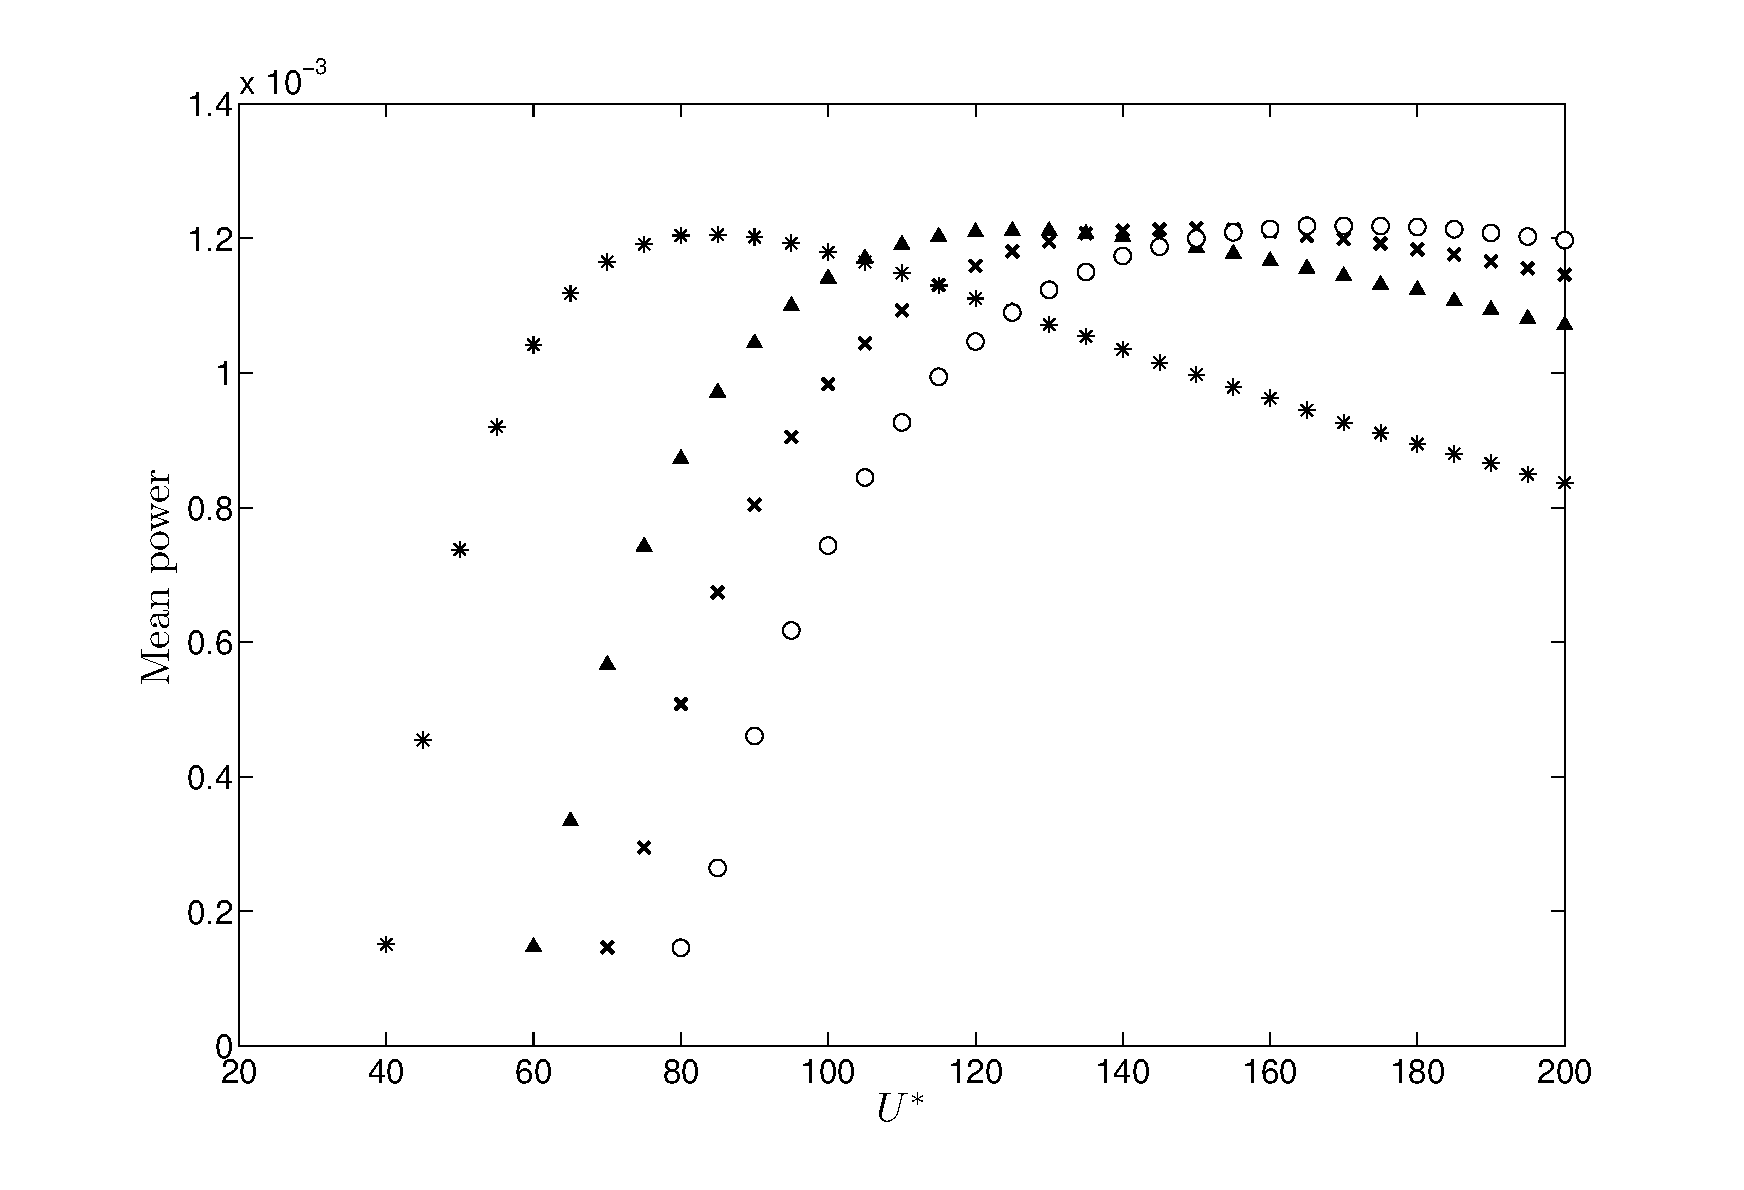
\includegraphics[width=0.8\linewidth]{../FnP/power_barrero_style_zeta_165}
\caption{Mean power vs. reduced velocity at different damping ratios at $m^*=20$. \ding{83} $ \zeta = 0.1$, \ding{58} $\zeta = 0.15$, \ding{115} $\zeta = 0.175$ and \ding{54} $\zeta = 0.2$, at Re = 165.}
\label{fig:power_barrero_style_zeta_165}
\end{figure}

\begin{figure}
\centering
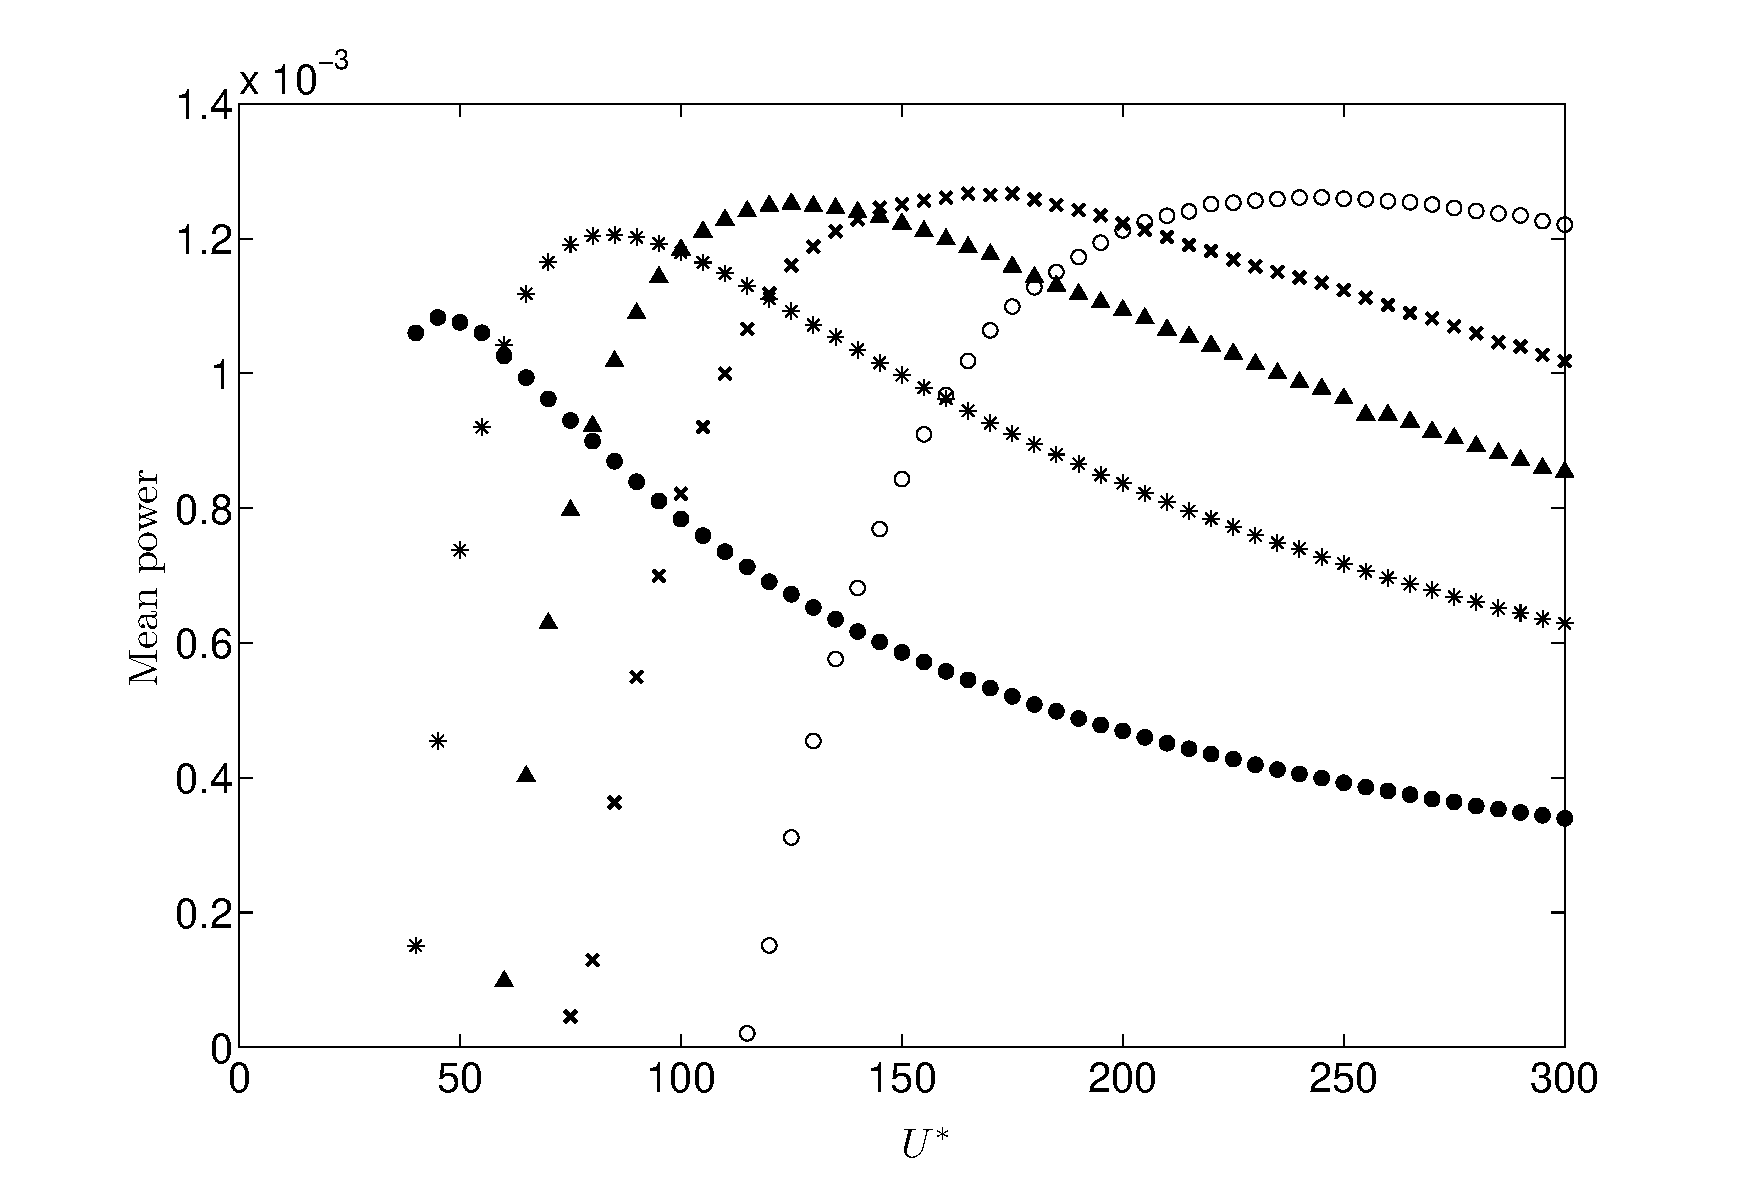
\includegraphics[width=0.8\linewidth]{../FnP/power_barrero_style_mstar_165}
\caption{Mean power vs. $U^*$ at different $m^*$ $\zeta=0.1$ (\ding{83} $m^*=20$, \ding{115} $m^*=30$, $\times$ $m^*=40$ and  $\circ$ $m^* = 60$,, at Re = 165)} 
\label{fig:power_barrero_style_mstar_165}
\end{figure}

\begin{figure}[htbp]
\centering
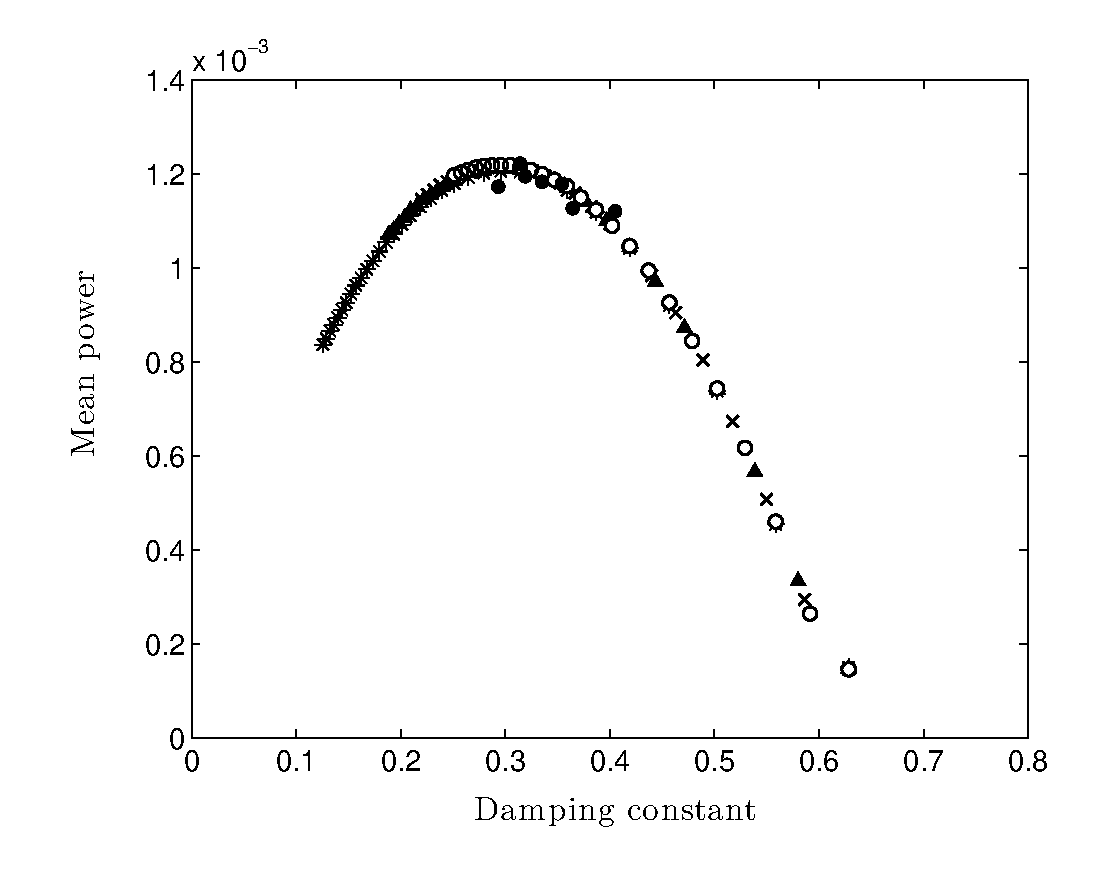
\includegraphics[width=0.7\textwidth]{../FnP/from_reynolds/mean_power_collapsed_c_with_FSI}
\caption{Mean power vs. damping constant at $m^*=20$. \ding{83} $ \zeta = 0.1$, \ding{115} $\zeta = 0.15$,   $\times$ $\zeta = 0.175$ and $\circ$ $\zeta = 0.2$ and \ding{108} FSI data at Re = 165 }
\label{fig:mean_power_collapsed_c_with_FSI}
\end{figure}



\begin{figure}
\centering
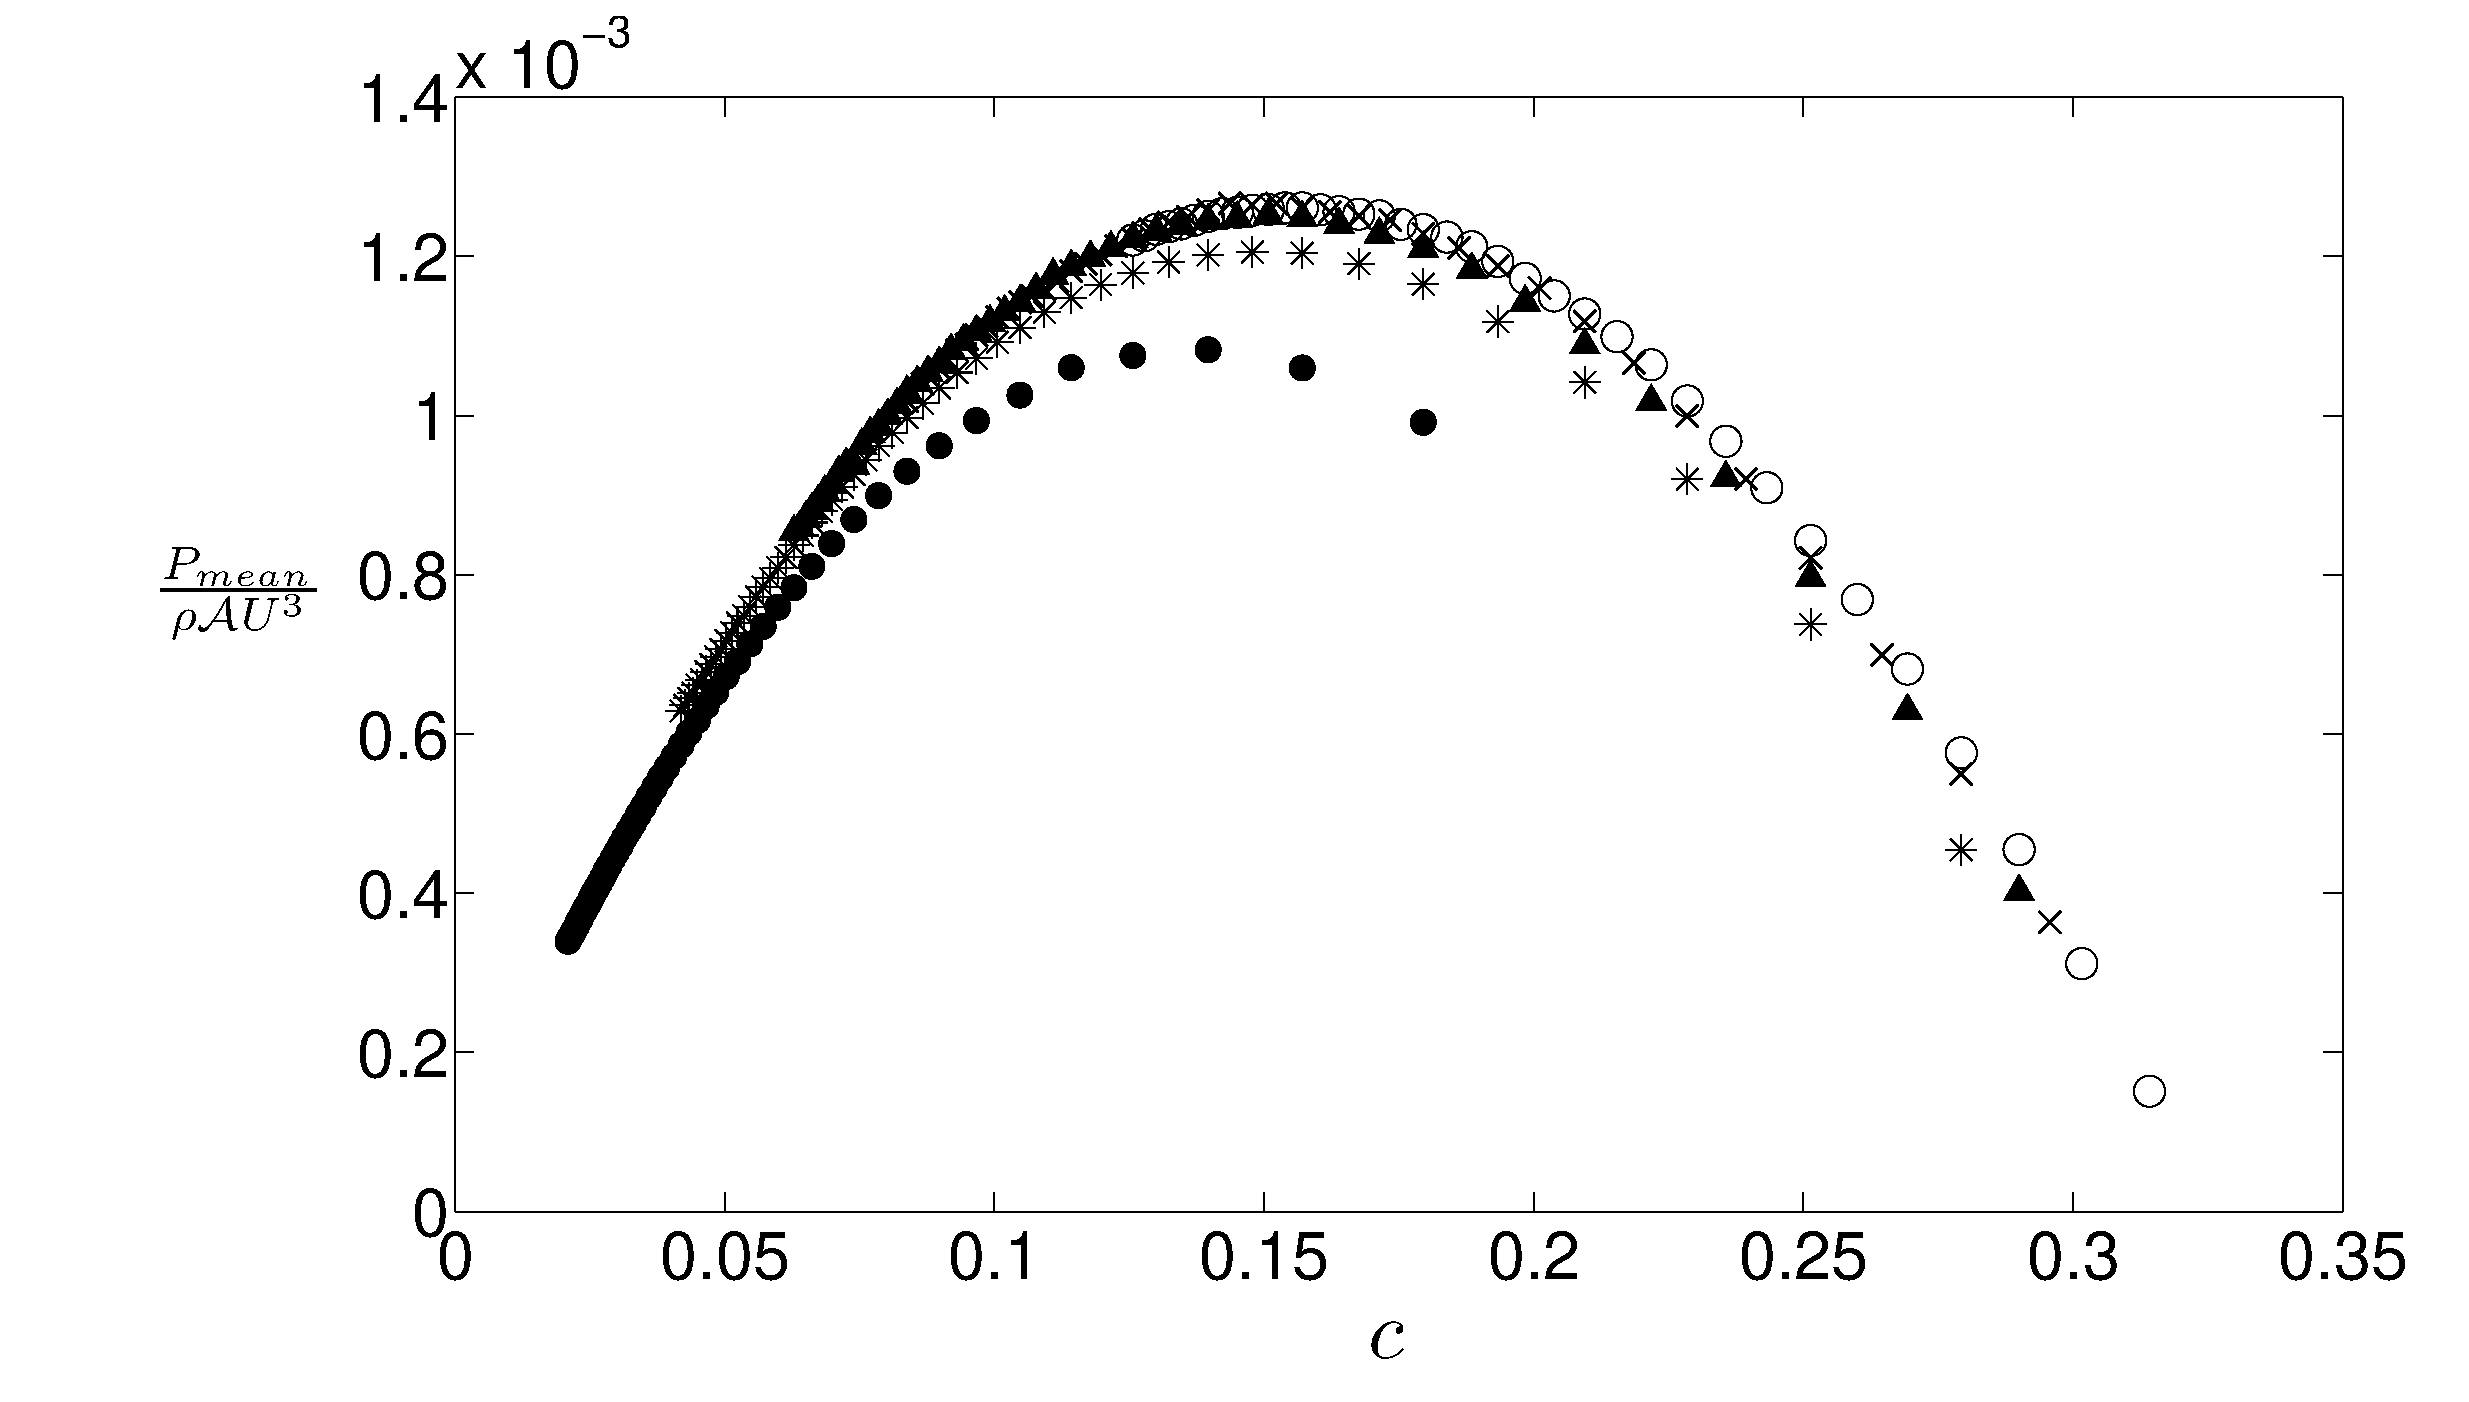
\includegraphics[width=0.8\linewidth]{../FnP/power_barrero_style_mstar_collapsed_165}
\caption{Mean power vs. damping ratio at different $m^*$ $\zeta=0.1$ (,\ding{108} $m^*=10$,\ding{83} $m^*=20$, \ding{115} $m^*=30$, $\times$ $m^*=40$ and  $\bigcirc$ $m^* = 60$, at Re = 165) } 
\label{fig:power_barrero_style_mstar_collapsed_165}
\end{figure}

\begin{figure}
\centering
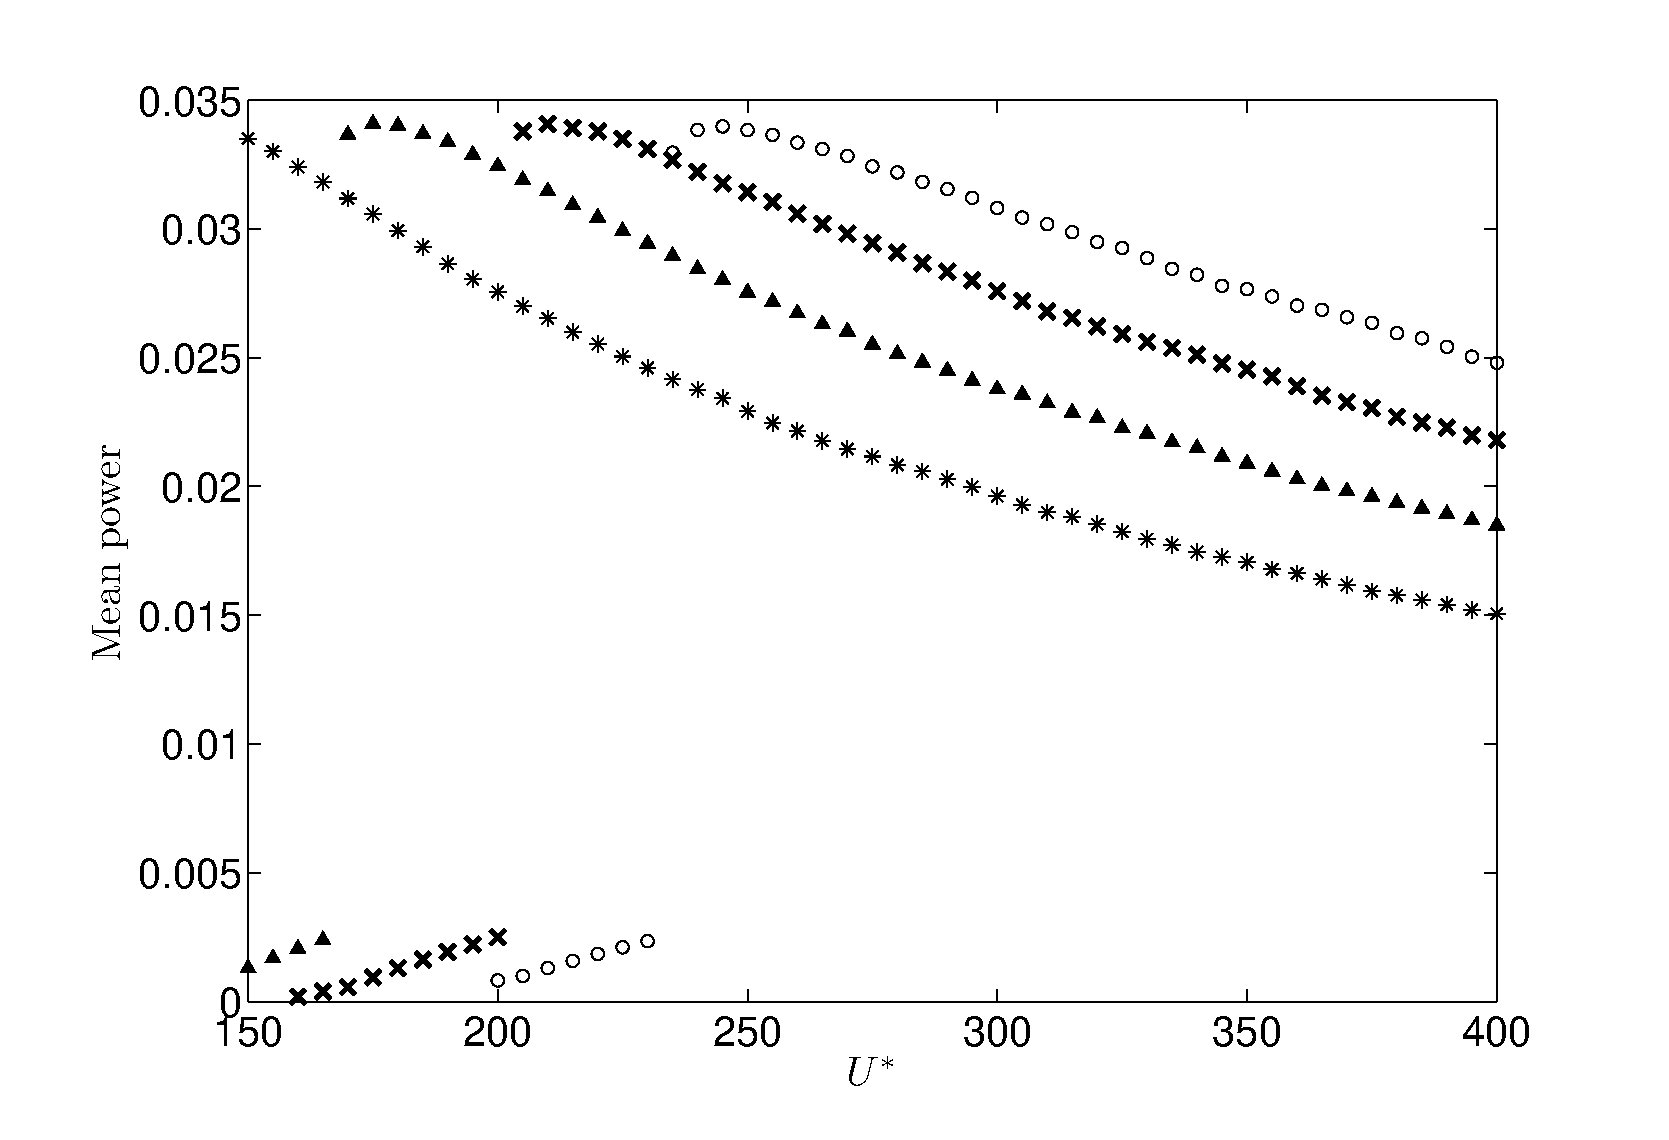
\includegraphics[width=0.7\linewidth]{../FnP/power_barrero_style_zeta_Park}
\caption{}
\label{fig:power_barrero_style_zeta_Park}
\end{figure}


 



\begin{figure}
\centering
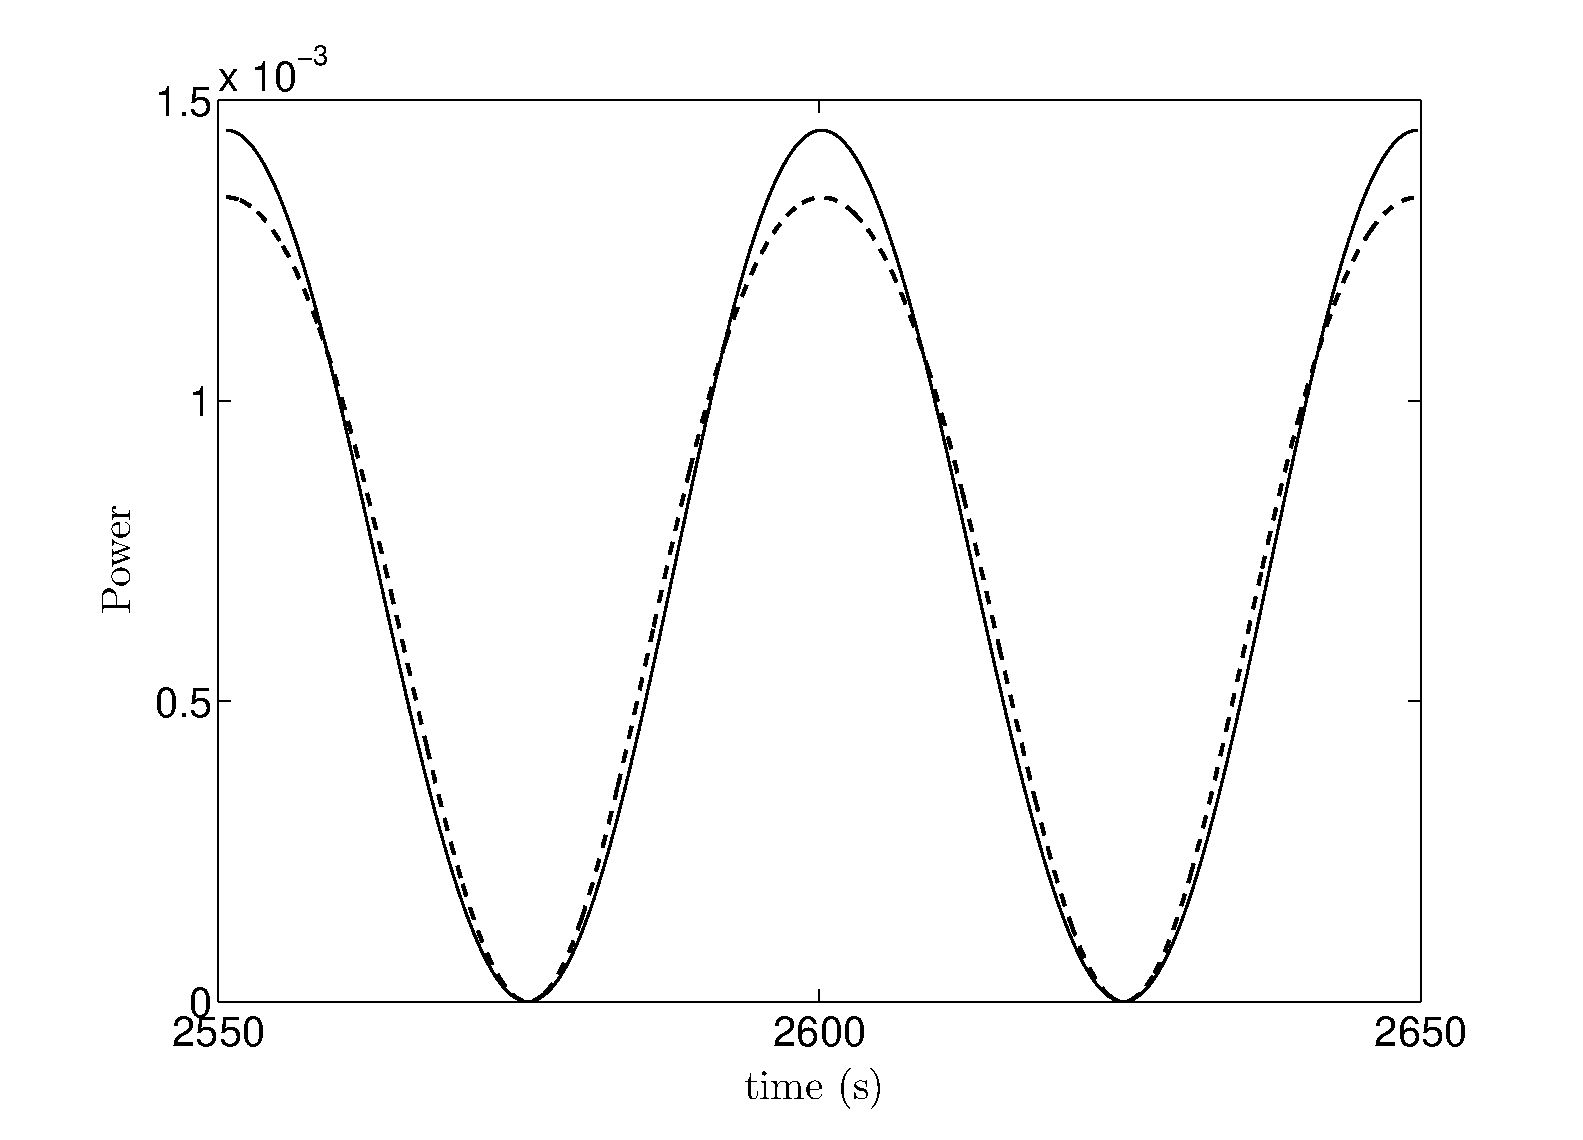
\includegraphics[width=0.7\linewidth]{../FnP/power_time_history_re165_95_0_1}
\caption{}
\label{fig:power_time_history_re165_95_0_1}
\end{figure}



\begin{figure}
\centering
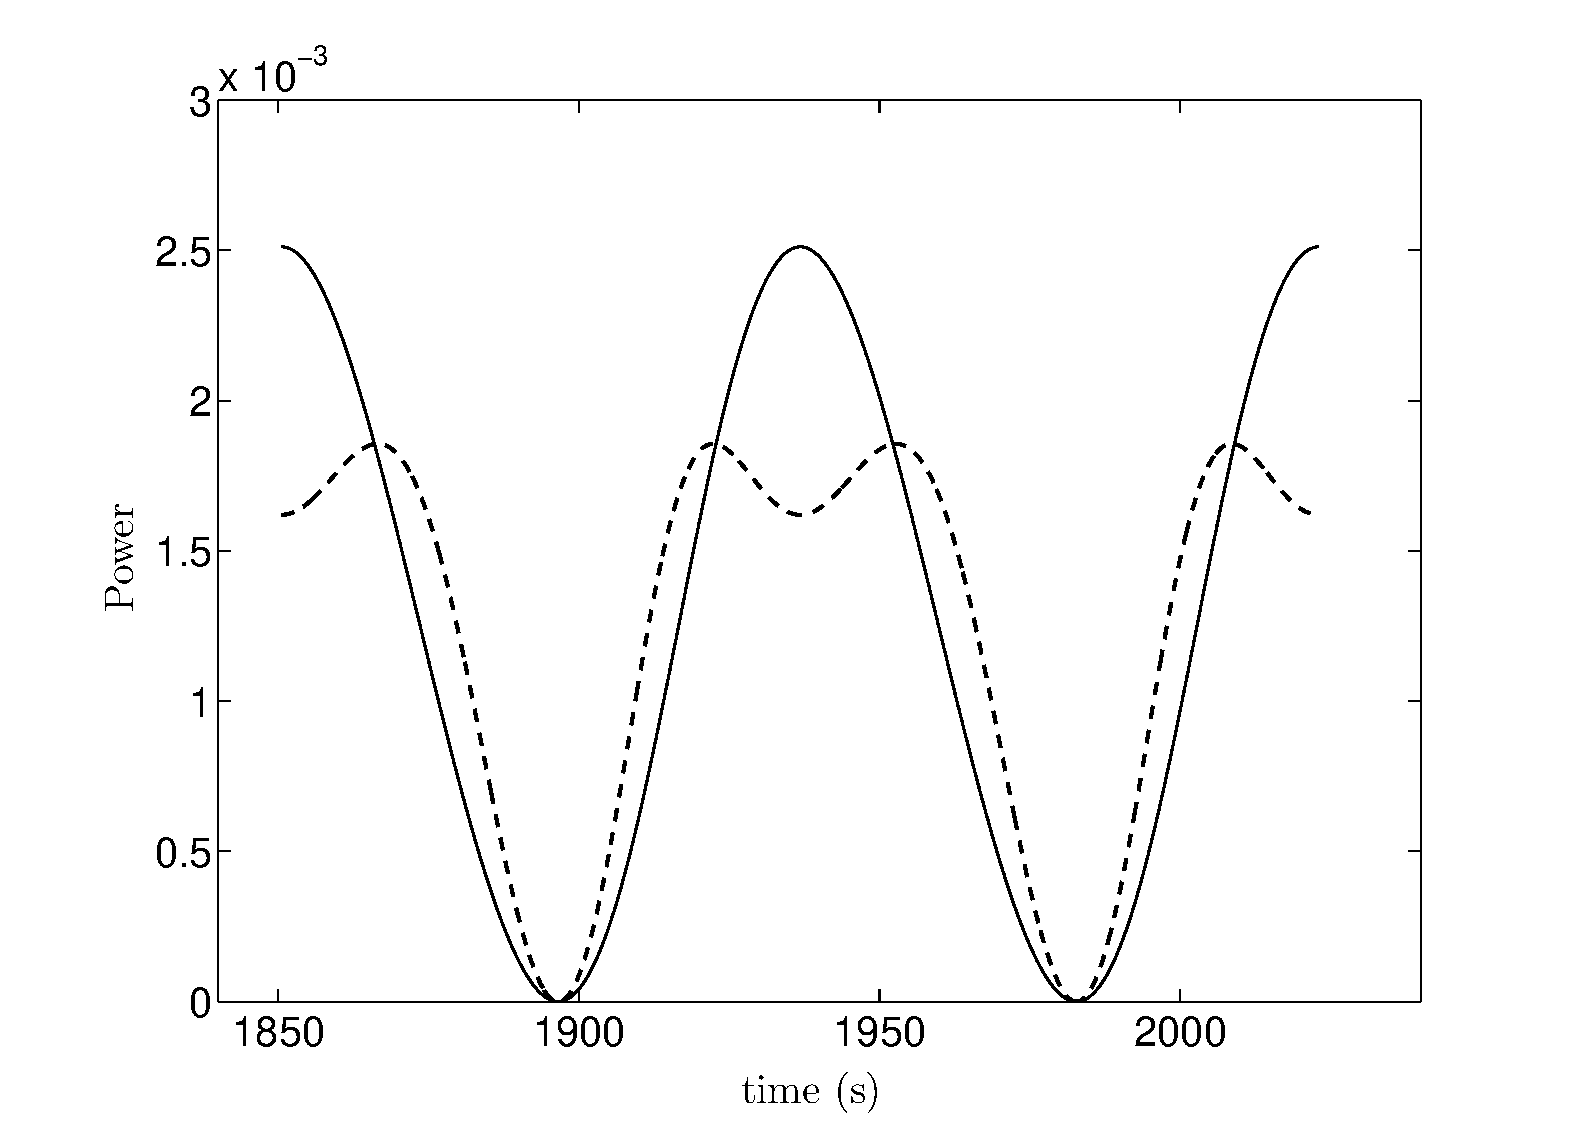
\includegraphics[width=0.7\linewidth]{../FnP/power_time_history_re165_165_0_1}
\caption{}
\label{fig:power_time_history_re165_85_0}
\end{figure}




\begin{figure}
\centering
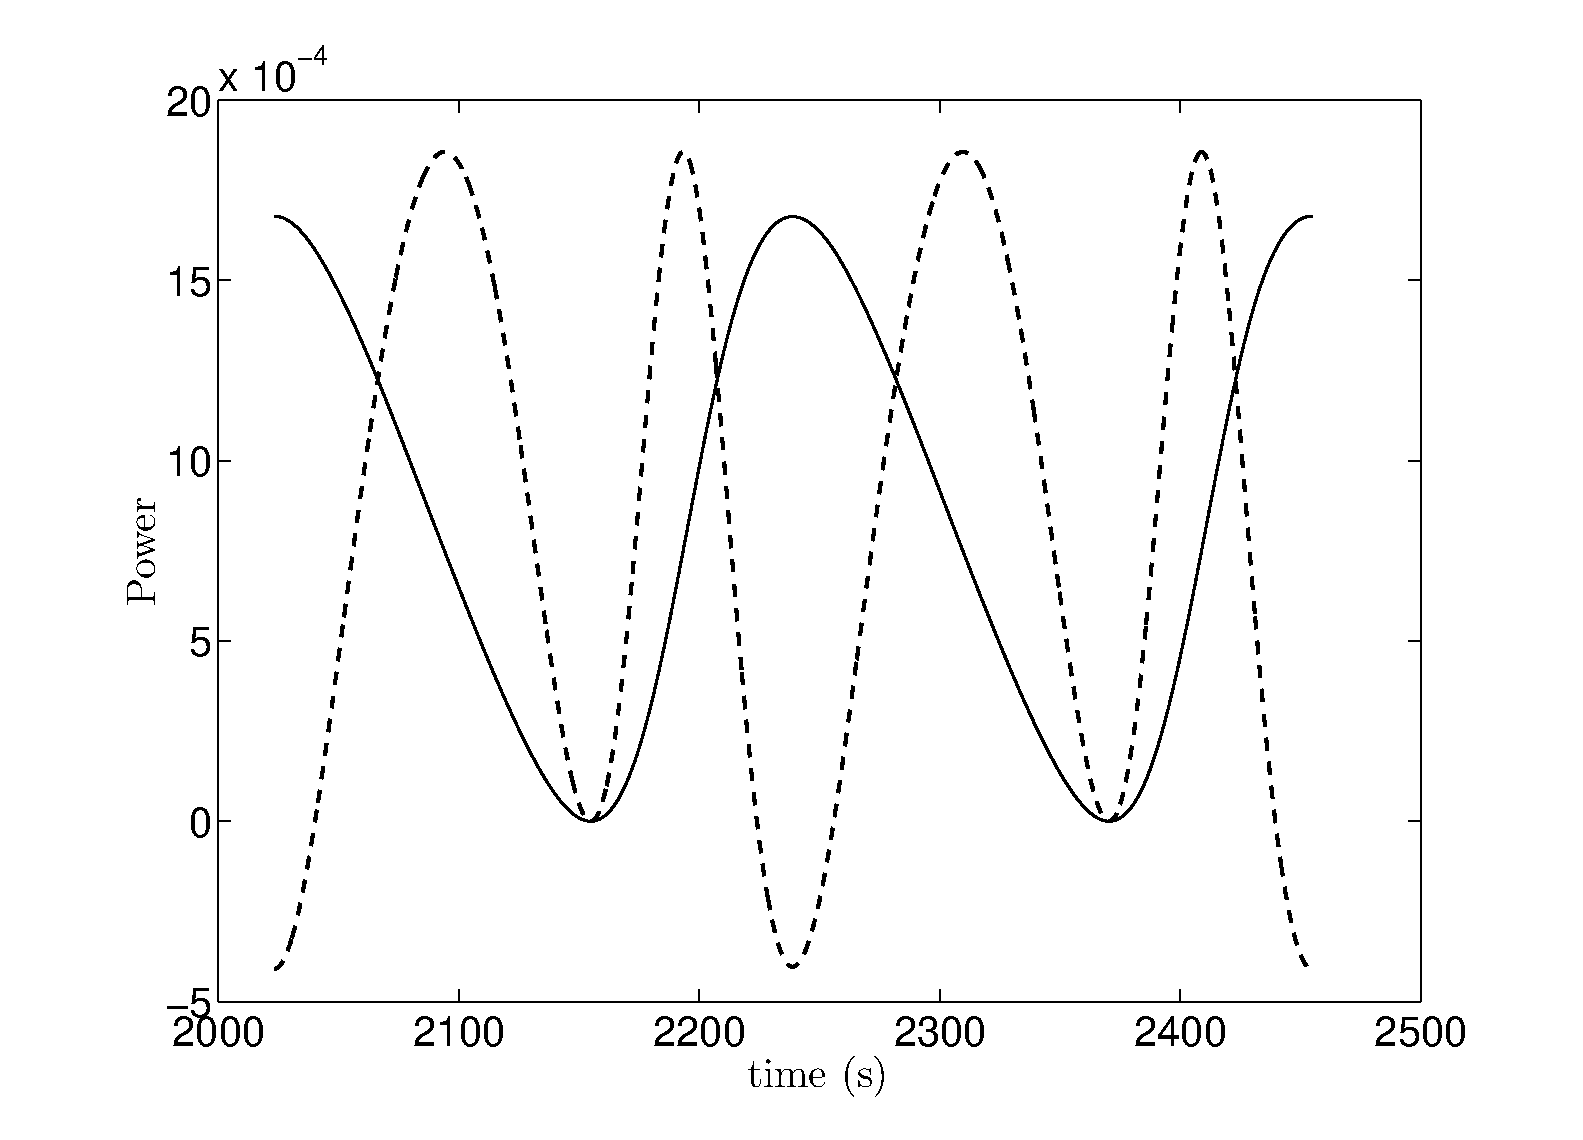
\includegraphics[width=0.7\linewidth]{../FnP/power_time_history_re165_400_0_1}
\caption{}
\label{fig:power_time_history_re165_400_0_1}
\end{figure}


\begin{figure}[htbp]
\centering
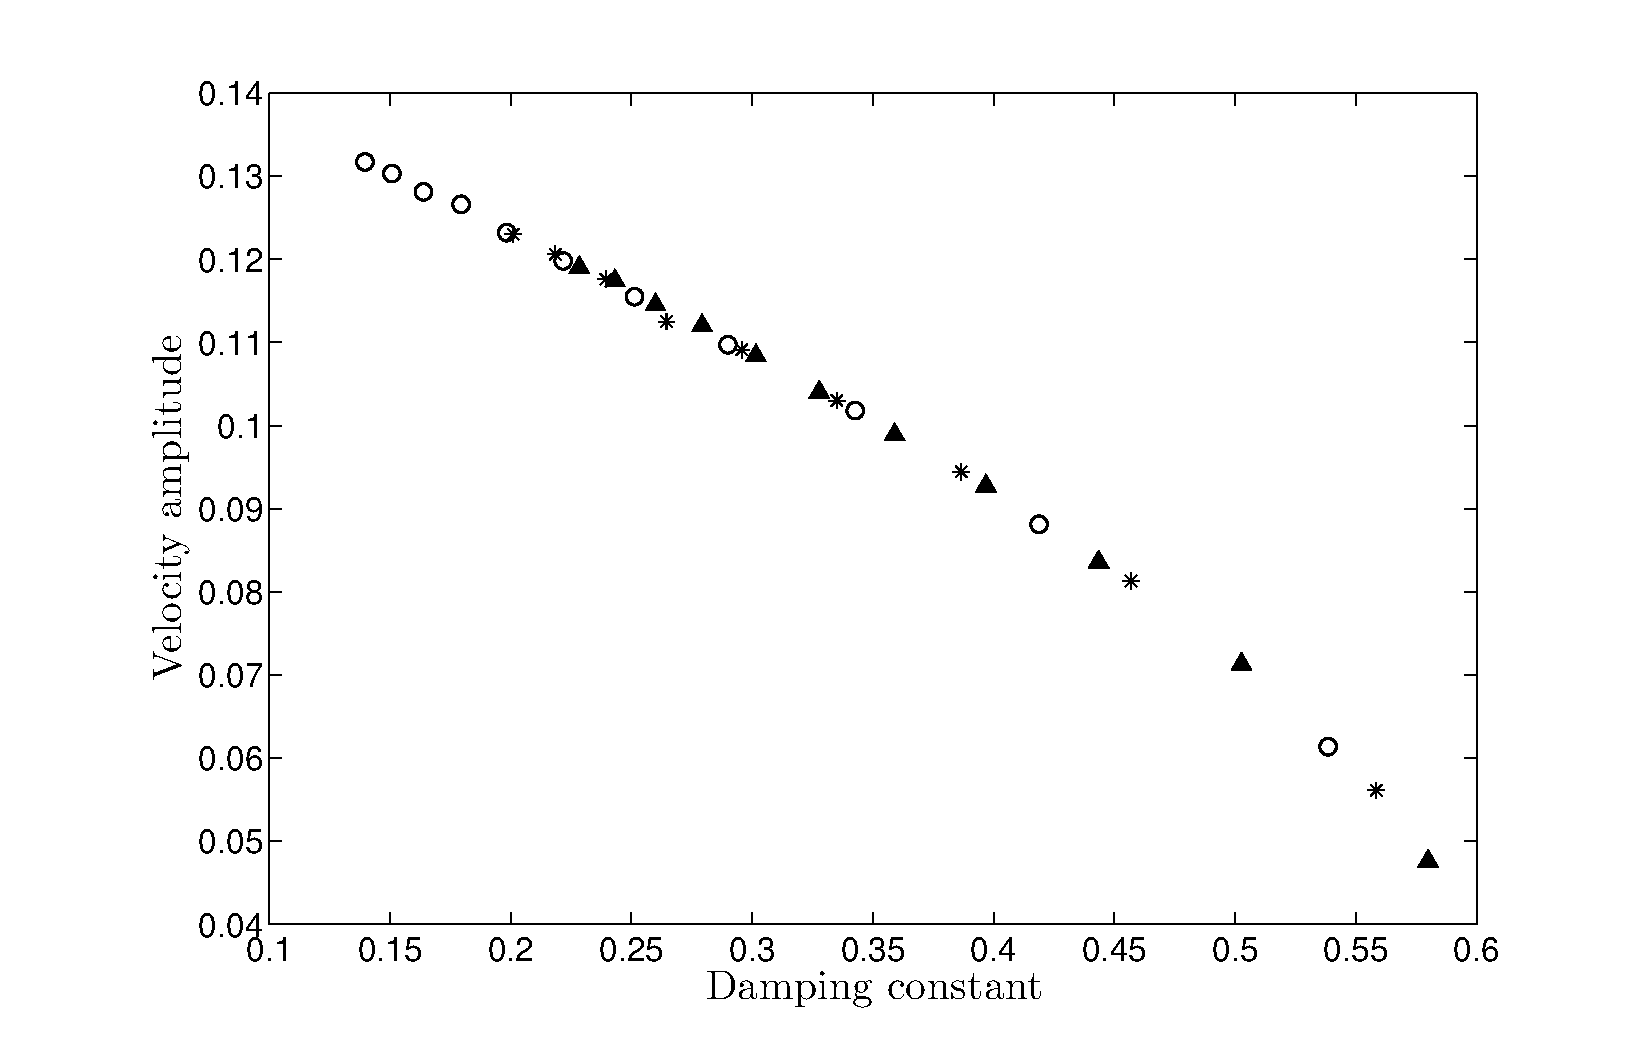
\includegraphics[width=0.7\linewidth]{../FnP/from_reynolds/velocity_amp_collapsed}
\caption{Velocity amplitude vs. damping constant at $m^*=20$. $\circ$ $\zeta = 0.075$, \ding{83} $ \zeta = 0.1$, \ding{115} and $\zeta = 0.15$, at Re = 165}
\label{velocity_amplitude_damping_constant_diff_zeta}
\end{figure}



\begin{figure}[htbp]
\centering
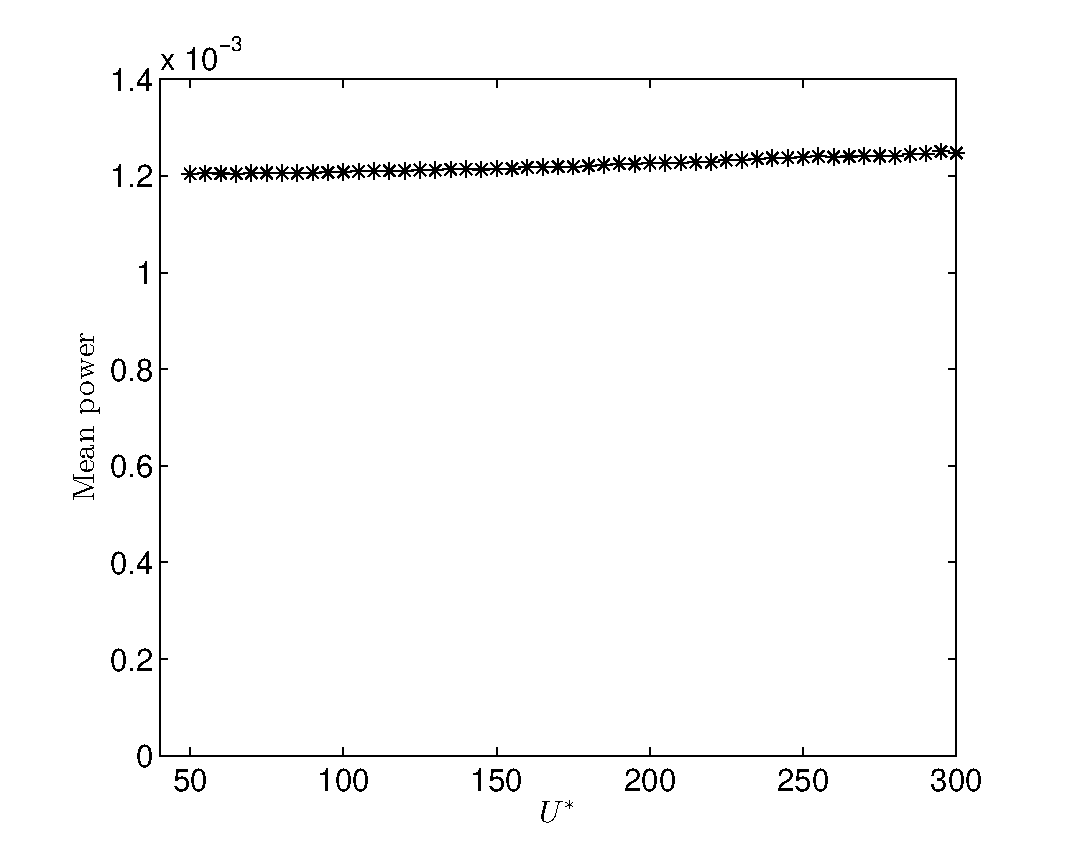
\includegraphics[width=0.7\textwidth]{../FnP/from_reynolds/constan_power_given_c}
\caption{Plot of mean power at  damping factor = 2.99}
\label{fig:constan_power_given_c}
\end{figure}


















